\chapter{Theoretical Background}
\label{Theoretical Background for GAN}
This chapter provides an overview of Generative Adversarial Networks (GANs), focusing on their core architecture, objective function, and training dynamics. It introduces the interplay between the generator and discriminator in the adversarial training process, as well as the Fréchet Inception Distance (FID) metric for evaluating the quality and diversity of generated images.



\section{Generative Adversarial Networks (GANs)}

Generative Adversarial Networks (GANs) were introduced by Goodfellow et al. in 2014 and have become a widely used approach in generative modeling. GANs consist of two neural networks: a generator (G) and a discriminator (D), trained simultaneously through an adversarial process. The generator is tasked with producing synthetic data samples, while the discriminator tries to distinguish between real and generated samples. This architecture leads to a game-like dynamic between the two networks, where the generator improves its ability to create realistic data while the discriminator becomes better at distinguishing real from fake data \citep{10.1109/taslp.2017.2761547}, \citep{10.1007/s10928-021-09787-4} and provide feedback to the generator, helping it to improve and generate more realistic samples over time \citep{10.48550/arxiv.1802.05637}.

\section{GAN Architecture}

The structure of GANs consists of two key components:
\begin{itemize}
    \item \textbf{Generator (G)}: The generator maps random noise \(z\) from a prior distribution, such as Gaussian or uniform, to synthetic data samples \(G(z)\) that aim to replicate real data distributions.
    \item \textbf{Discriminator (D)}: The discriminator receives input data, which can be either real data \(x\) or generated data \(G(z)\), and outputs the probability that the data is real. The discriminator is trained to classify real samples as real and generated samples as fake \citep{10.48550/arxiv.1802.05637}.
\end{itemize}

The following figure illustrates the GAN architecture, where the generator produces synthetic data, and the discriminator learns to differentiate real from fake data.

\begin{figure}[H]
    \centering
    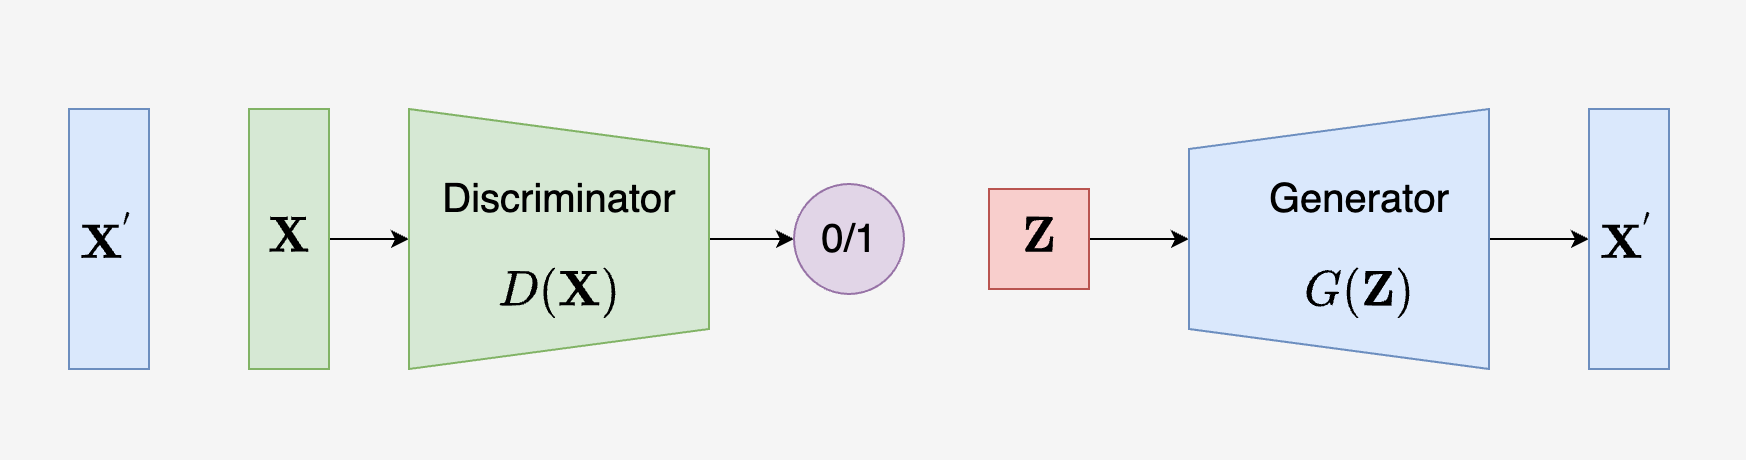
\includegraphics[width=0.9\textwidth]{./Images/GAN_structure.jpg}
    \caption{GAN Architecture.}
    \label{fig:GAN_structure}
\end{figure}


\section{Objective Function of GAN}

The training of GANs involves optimizing two neural networks simultaneously through a minimax game. The objective function is defined as follows:

\begin{equation}
    \min_{G} \max_{D} V(D, G) = \mathbb{E}_{x \sim p_{data}(x)} [\log D(x)] + \mathbb{E}_{z \sim p_{z}(z)} [\log(1 - D(G(z)))].
\end{equation}
where :
\begin{itemize}
    \item \(z \sim p_z(z)\): The distribution from which the noise \(z\) is sampled. The generator transforms this noise into complex, high-dimensional data.
    \item \(x \sim p_{data}(x)\): A sample \(x\) drawn from the true data distribution \(p_{data}(x)\).
    \item \(D(G(z))\): The discriminator's prediction for generated data \(G(z)\).
    \item \(D(x)\): The discriminator's prediction for real data \(x\).
    \item \(\mathbb{E}_{x \sim p_{data}(x)}[\log D(x)]\): The expectation of \(\log D(x)\) over the real data distribution.
    \item \(\mathbb{E}_{z \sim p_z(z)}[\log(1 - D(G(z)))]\): The expectation of \(\log(1 - D(G(z)))\) over the noise distribution.
\end{itemize}

\subsection{Discriminator's Loss Function}

The discriminator’s loss function measures its ability to distinguish between real and generated data. It is expressed as:

\begin{equation}
    \label{eq:discriminator_loss}
    \mathcal{L}_D = -\mathbb{E}_{x \sim p_{\text{data}}(x)} [\log D(x)] - \mathbb{E}_{z \sim p_z(z)} [\log(1 - D(G(z)))].
\end{equation}

The discriminator minimizes this loss function to improve its ability to classify real and generated data correctly.

\subsection{Generator's Loss Function}

The generator’s loss function is designed to encourage it to generate data that can fool the discriminator. It is given by:

\begin{equation}
    \label{eq:generator_loss}
    \mathcal{L}_G = -\mathbb{E}_{z \sim p_z(z)} [\log D(G(z))].
\end{equation}

The generator minimizes this loss function to produce data that the discriminator classifies as real.

\subsection{Modification for Vanishing Gradient Problem}

To address the vanishing gradient problem during GAN training, the generator’s loss is often modified. The original form \(\log(1 - D(G(z)))\) can result in small gradients when the discriminator accurately identifies fake data. Therefore, the alternative loss function for the generator is:

\begin{equation}
    \label{eq:new_generator_loss}
    \mathcal{L}_G = \mathbb{E}_{z \sim p_z(z)} [-\log(D(G(z)))].
\end{equation}

This modification ensures larger gradients and more stable training.

\begin{figure}[H]
    \centering
    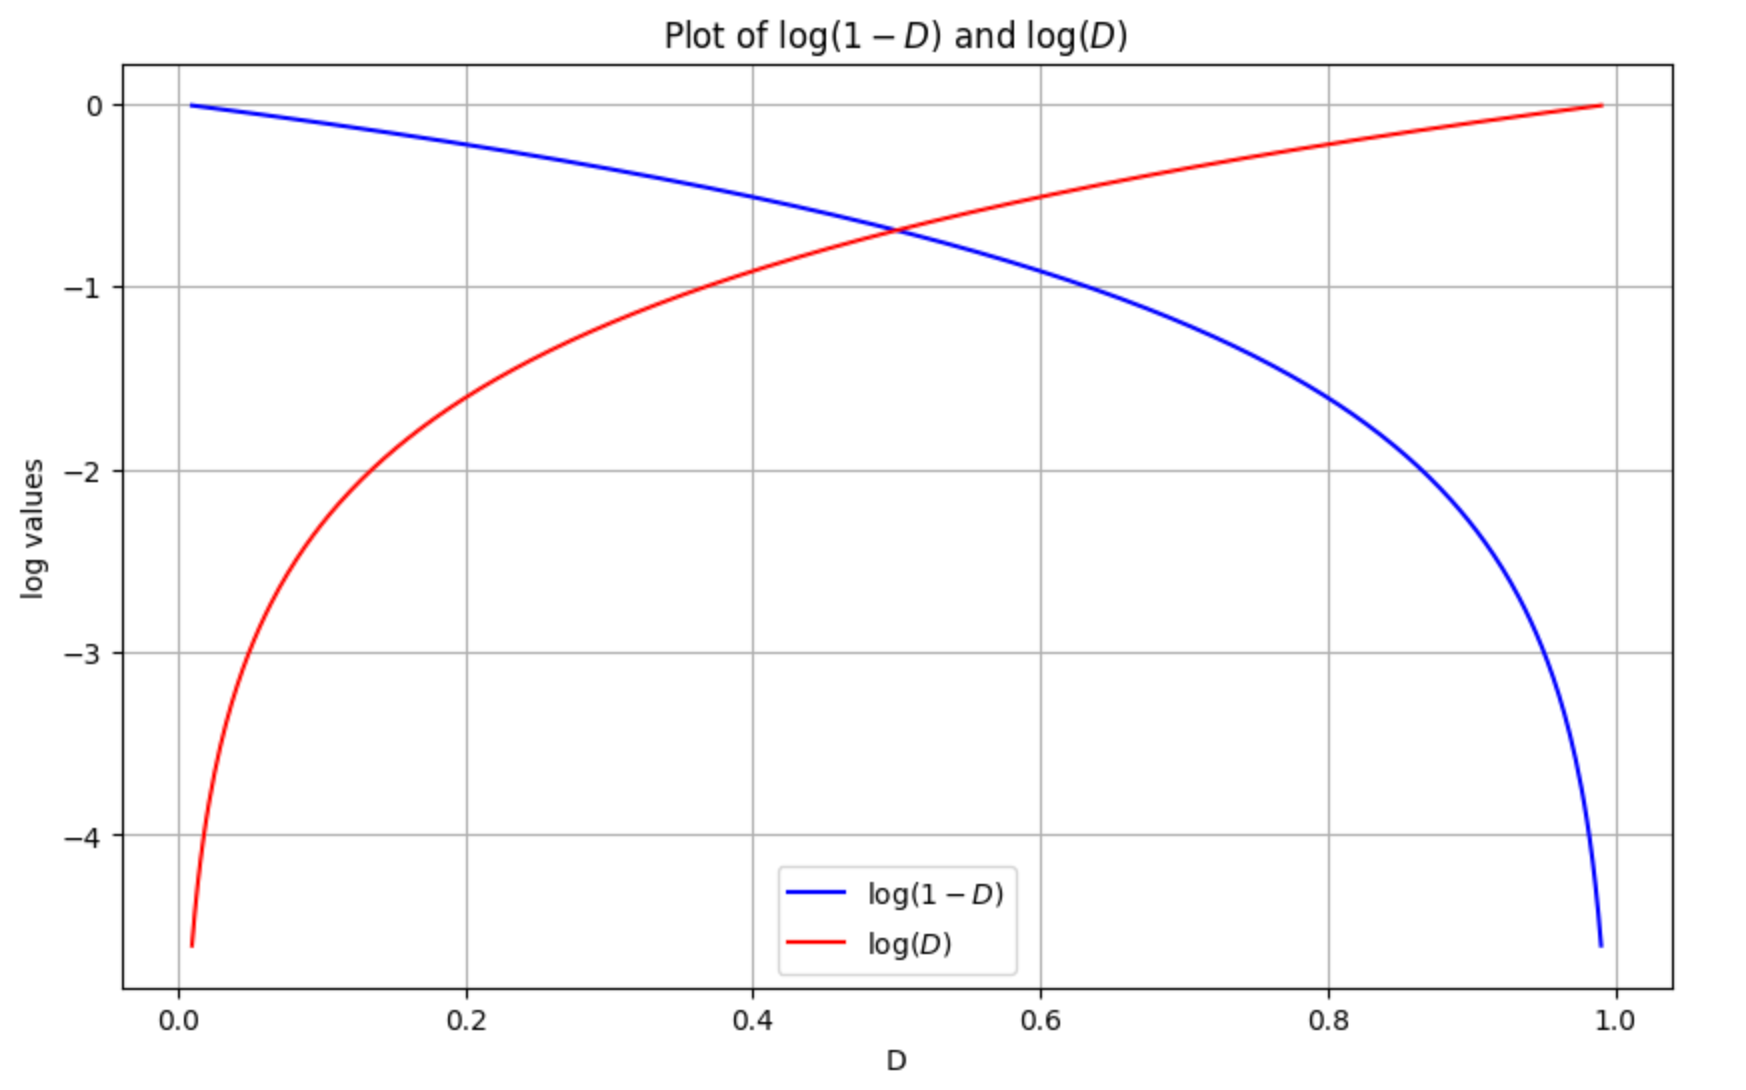
\includegraphics[width=0.8\textwidth]{./Images/log_gunction.jpg}
    \caption{Comparison of $\log(1 - D)$ and $-\log(D)$.}
    \label{fig:log_function}
\end{figure}



\section{GAN Training Process}

During the training process of the GAN model, the generator and the discriminator are in constant competition. 
The generator aims to produce increasingly realistic samples to deceive the discriminator, while the discriminator 
works to accurately distinguish between real and generated samples. Initially, the generator produces samples 
that are of low quality and deviate significantly from the real data, as illustrated by the blue sine wave in 
Figure (a). As training progresses, the generator improves, and the generated samples become more refined, 
as shown by the smoother blue lines in Figures (b) and (c). Simultaneously, the distribution of the real samples 
and generated samples gradually align, and finally, in the optimal state represented by Figure (d), 
$p_{data}(x) = p_g(x)$, meaning that the generated samples closely match the real samples. Throughout the 
training process, the distribution of the generated samples transitions from an initially noisy and scattered state 
to one that closely mirrors the real data distribution, indicating a significant enhancement in the quality 
of the generated samples.

\subsection{Distribution Changes During GAN Training}
A simaple diagram show how distribution change in GAN training.

\begin{figure}[H]
    \centering
    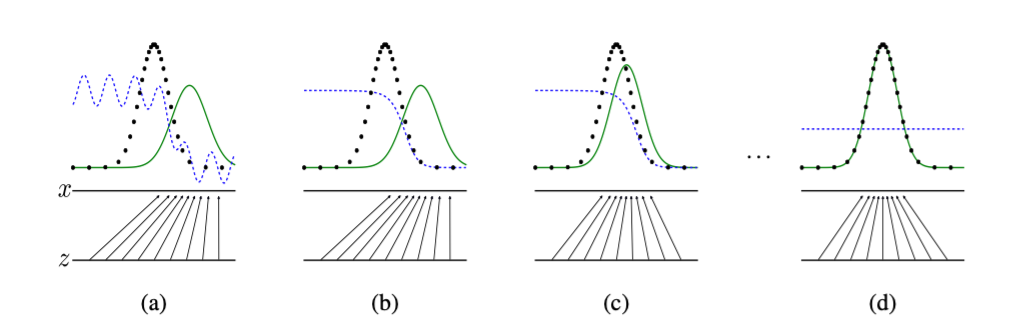
\includegraphics[width=1.2\linewidth]{./Images/data_distribution.jpg}
    \caption{ Diagram of GAN's Training Process. 
    The green curve represents the distribution of generated samples. Initially, the generated samples may differ significantly from the real samples. As training progresses, the generated samples' distribution gradually approaches the real samples.
    The black dots represent the distribution of real samples, which remains unchanged throughout the training process and represents the target distribution.
    The blue dashed line represents the discriminator's output probability distribution. At the beginning of training, the discriminator can easily distinguish between real and generated data, resulting in a strong classification boundary. As training progresses and the generated data becomes more realistic, the discriminator's ability to differentiate between the two distributions weakens. Eventually, the discriminator's output approaches 0.5, indicating it can no longer effectively distinguish between real and generated data.
    The lines labeled $x$ and $z$ below represent the distribution of samples in the latent space. During GAN training, samples from the latent space $z$ are mapped to the data space $x$ through the generator.
    }
    \label{fig:gan_training_process}
    \vspace{1pt} % Vertical space, optional
    \small{Source: \cite{goodfellow2014generative}}
\end{figure}

As training progresses, the samples generated by the generator gradually become indistinguishable from the real data, leading to a minimized error between the two distributions. Initially, the generated samples exhibit significant differences from the real data, starting from a noisy and dispersed state. However, over time, the generator learns to map the latent space to the real data distribution more accurately. This results in the generated samples converging toward the real data distribution, ultimately aligning closely with the target distribution.


\subsection{Mathematical Formulation during GAN Training}


1. Problem Setup

In a Generative Adversarial Network (GAN), the objective is to train a generator \( G \) and a discriminator \( D \) 
to generate data that resembles the real data distribution. The objective function to be maximized is given by:

\begin{equation}
    V(D, G) = \mathbb{E}_{x \sim p_{\text{data}}(x)} [\log D(x)] + \mathbb{E}_{z \sim p_{z}(z)} [\log (1 - D(G(z)))].
\end{equation}

2. Rewriting the Objective Function

First, the objective function is rewritten in integral form:

\begin{equation}
    V(D, G) = \int p_{\text{data}}(x) \log D(x) \, dx + \int p_{z}(z) \log (1 - D(G(z))) \, dz.
\end{equation}

By changing variables $x' = G(z)$, the generated data is represented as $x'$, which corresponds to samples produced by the generator $G$. This allows the second term to be rewritten as an integral over the generated data distribution $p_g(x)$. The integral now reflects the contribution of the generated samples to the objective function.

\begin{equation}
    \int p_g(x) \log (1 - D(x)) \, dx.
\end{equation}

Thus, the objective function becomes:

\begin{equation}
    V(D, G) = \int \left[ p_{\text{data}}(x) \log D(x) + p_g(x) \log (1 - D(x)) \right] dx.
\end{equation}

3. Deriving the Optimal Discriminator

To find the optimal discriminator \( D^* \), it needs to take the derivative of the objective function with respect to \( D(x) \) and set it to zero.

Let:

\begin{equation}
    f(D(x)) = p_{\text{data}}(x) \log D(x) + p_g(x) \log (1 - D(x)).
\end{equation}

Taking the derivative with respect to \( D(x) \):

\begin{equation}
    \frac{d}{dD(x)} f(D(x)) = \frac{p_{\text{data}}(x)}{D(x)} - \frac{p_g(x)}{1 - D(x)}.
\end{equation}

Setting the derivative to zero:

\begin{equation}
    \frac{p_{\text{data}}(x)}{D(x)} = \frac{p_g(x)}{1 - D(x)}
    \label{eq:derivative_to_zero}
\end{equation}

Solving equation \eqref{eq:derivative_to_zero}:

\begin{equation}
    D(x) = \frac{p_{\text{data}}(x)}{p_{\text{data}}(x) + p_g(x)}.
\end{equation}

4. Optimal Discriminator Formula

Therefore, the optimal discriminator \( D^* \) is given by:

\begin{equation}
    D^*(x) = \frac{p_{\text{data}}(x)}{p_{\text{data}}(x) + p_g(x)}.
\end{equation}


\begin{itemize}
    \item When $p_{\text{data}}(x)$ is much larger than $p_g(x)$, $D^*(x) \approx 1$, indicating that the data point is almost certainly from the real data.
    
    \item When $p_{\text{data}}(x)$ is much smaller than $p_g(x)$, $D^*(x) \approx 0$, indicating that the data point is almost certainly from the generated data.
    
    \item When $p_{\text{data}}(x)$ is close to $p_g(x)$, $D^*(x) \approx 0.5$, indicating that the discriminator cannot confidently determine whether the data point is real or generated, giving each a 50\% probability.
\end{itemize}

5. Verifying the Optimal Discriminator

To verify that this \( D^* \) maximizes the objective function, substitute \( D^* \) back into the objective function:

\begin{equation}
    V(D^*, G) = \int \left[ p_{\text{data}}(x) \log \left( \frac{p_{\text{data}}(x)}{p_{\text{data}}(x) + p_g(x)} \right) + p_g(x) \log \left( 1 - \frac{p_{\text{data}}(x)}{p_{\text{data}}(x) + p_g(x)} \right) \right] dx.
\end{equation}

Since:

\begin{equation}
    1 - D^*(x) = 1 - \frac{p_{\text{data}}(x)}{p_{\text{data}}(x) + p_g(x)} = \frac{p_g(x)}{p_{\text{data}}(x) + p_g(x)},
\end{equation}

substituting this in:

\begin{equation}
    V(D^*, G) = \int \left[ p_{\text{data}}(x) \log \left( \frac{p_{\text{data}}(x)}{p_{\text{data}}(x) + p_g(x)} \right) + p_g(x) \log \left( \frac{p_g(x)}{p_{\text{data}}(x) + p_g(x)} \right) \right] dx.
\end{equation}

This objective function represents the negative of the cross-entropy, which is maximized when $D(x) = D^*(x)$. When $D(x) = 0.5$, the discriminator cannot distinguish between real and generated data, indicating that the generator has produced samples that closely resemble the real data. Maximizing the negative cross-entropy aligns the generated data distribution with the real data distribution.

6. Conclusion

Through the above derivation, it has shown that given the generator \( G \), the optimal form of the discriminator \( D \) is:

\begin{equation}
    D^*(x) = \frac{p_{\text{data}}(x)}{p_{\text{data}}(x) + p_g(x)}.
\end{equation}

This demonstrates that the optimal discriminator \( D^* \) outputs the probability that the input data comes from the 
real data distribution. 
This formula provides a theoretical foundation for training GANs, guiding the updates to the generator \( G \) so that 
its generated data gradually approaches the real data distribution.


\section{Evaluating GAN Performance}


Fréchet Inception Distance (FID) is a metric commonly used in Generative Adversarial Network (GAN) models 
to quantify the dissimilarity between two image distributions \citep{10.48550/arxiv.2203.06026}. 
It measures the distance between the distributions of real images and generated images, providing 
a numerical assessment of the quality of generated images. FID has gained prominence in evaluating 
the performance of GANs due to its ability to capture both the quality and diversity of generated images \citep{10.3390/app12157599}.
The following is the objective function for FID:


\begin{equation}
    \text{FID} = || \mu_r - \mu_g ||^2 + \text{Tr}(\Sigma_r + \Sigma_g - 2(\Sigma_r \Sigma_g)^{1/2})
\end{equation}


\begin{equation}
    \mu_r = \frac{1}{N} \sum_{i=1}^{N} f(x_i), \quad \Sigma_r = \frac{1}{N} \sum_{i=1}^{N} (f(x_i) - \mu_r)(f(x_i) - \mu_r)^T
\end{equation}

\begin{equation}
    \mu_g = \frac{1}{M} \sum_{i=1}^{M} f(G(z_i)), \quad \Sigma_g = \frac{1}{M} \sum_{i=1}^{M} (f(G(z_i)) - \mu_g)(f(G(z_i)) - \mu_g)^T
\end{equation}

where:

\begin{itemize}
    \item \(\mu_r \text{ and } \mu_g\): The feature means of the real and generated images, respectively.
    \item \(\Sigma_r \text{ and } \Sigma_g\): The feature covariance matrices of the real and generated images, respectively.
    \item \(\text{Tr}\): The trace (the sum of the diagonal elements of the matrix).
    \item \(f\): The feature extraction function, which extracts feature vectors from images using the Inception network. These feature vectors are used to compute the mean and covariance for both real and generated images.
\end{itemize}

A lower FID value indicates that the distribution of the generated images is closer to that of real images, 
reflecting higher quality and diversity in the generated images \citep{10.1117/12.2673366}. 
Specifically, a FID value below 10 is considered to represent very high-quality generated images, 
while values between 10 and 50 indicate good quality, and values above 50 suggest average or poor quality \citep{10.1117/12.2673366}.



\section{Limitations of Accuracy in Evaluating GANs}
Accuracy is not suitable for evaluating GANs because accuracy is an indicator of classification tasks, 
which is used to measure the prediction accuracy of the model in classification tasks, and cannot 
measure the quality and diversity of generated data. In generation tasks, there is no clear 
"correct answer" and the generated data has no "real label", so it is impossible to directly 
compare the correspondence between the generated data and a real sample. 

The following is a result for a standard GANs model with high accuracy but generate low quality images.


\begin{figure}[H]
    \centering
    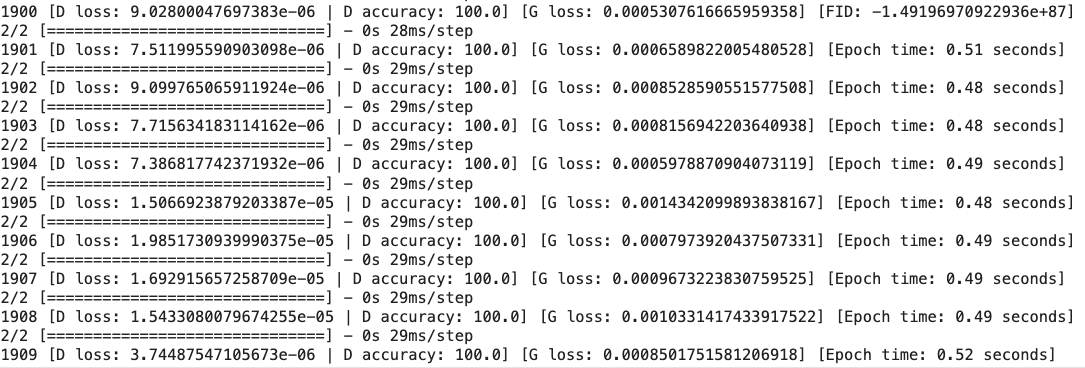
\includegraphics[width=1.2\linewidth]{./Images/model_accuracy.jpg}
    \caption{GAN Training Accuracy over Epochs}
    \label{fig:my_picture}
\end{figure}

\begin{figure}[H]
    \centering
    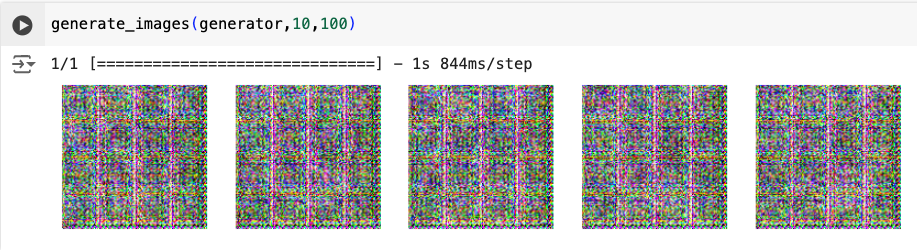
\includegraphics[width=1.2\linewidth]{./Images/generate_images.jpg}
    \caption{Generated Images from GAN}
    \label{fig:my_picture}
\end{figure}


FID (Fréchet Inception Distance) quantifies the difference between generated data and real 
data by comparing their distribution in the Inception network feature space. FID takes into 
account the overall distribution of generated data and real data, and can reflect the quality 
and diversity of generated data. A low FID value indicates that the distribution of generated 
data is very close to the distribution of real data, that is, the generated data is both realistic 
and diverse, so FID is a more suitable indicator for evaluating the performance of generative models.